\subsection{Impact of NetShaper on End Host Application Performance}
\label{subsec:netshaper-evaluation-http-reqs}

To determine if NetShaper throttles the performance of the end-host applications, we examine the behaviour of an HTTP server and client application pair.
We configure Nginx to serve a static HTTP file, which is crafted such that the response payload will be exactly 1460 bytes (i.e., the default MSS) to ensure that the request-response rate is not throttled due to the server serving larger files, which take more time to transmit.

We increase the request rate until the response rate is less than the request rate~
\footnote{wrk2 can spawn multiple clients and threads. Each client can send upto 2200 req/s on our setup. We scale the number of clients and threads to achieve the target request rate.}.
As we can see in \Cref{fig:netshaper-eval-http-reqs}, the client achieves 470k req/s without NetShaper.
However, increasing the request rate beyond 350k req/s negatively impacts the latency experienced by the clients, and the latency rises from less than 1ms to more than 1000ms (see \Cref{fig:netshaper-eval-http-reqs-latency}).
As such, we determine that the server is saturated at around 350k req/s.
NetShaper maintains the 350k req/s rate and even achieves slightly more at 380k req/s.
However, at 380k req/s, the \textit{QUIC worker} thread saturates and consumes 100\% of the CPU, thus not being able to achieve higher throughput.


\begin{figure}[!htb]
    \centering
    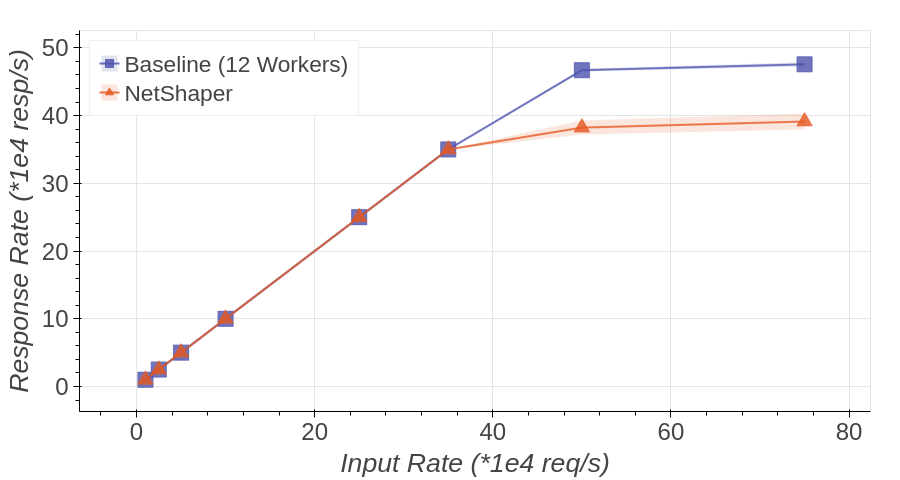
\includegraphics[width=\columnwidth]{figures/netshaper/evaluation/http_reqs.png}
    \caption{NetShaper's impact on Nginx Server Request Rate}
    \label{fig:netshaper-eval-http-reqs}
\end{figure}

\begin{figure}[!htb]
    \centering
    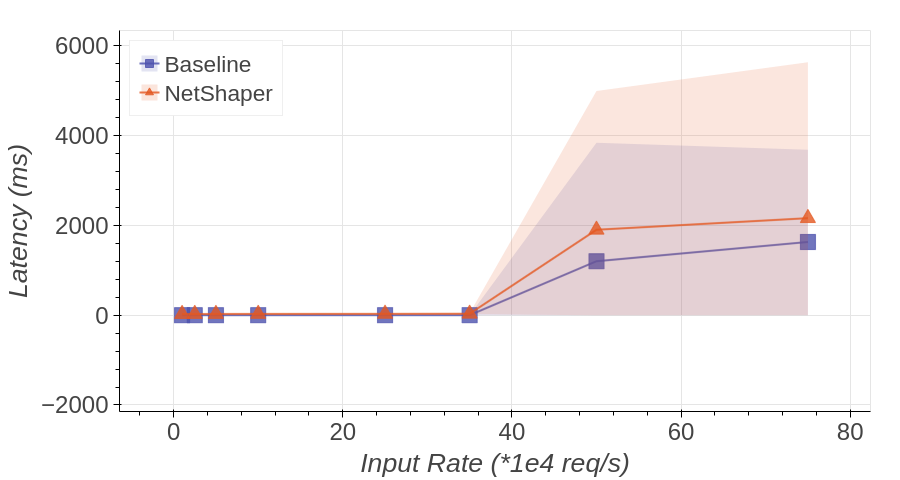
\includegraphics[width=\columnwidth]{figures/netshaper/evaluation/http_reqs_latency.png}
    \caption{Nginx Server Latency for Different Input Request Rates}
    \label{fig:netshaper-eval-http-reqs-latency}
\end{figure}